\باب{سوالات}

\حصہء{ترسیلی تار}
%===================
\ابتدا{سوال}
ترسیلی تار کے مستقل \عددی{R=\SI{20}{\ohm\per\meter}}، \عددی{L=\SI{4}{\micro\henry\per\meter}}، \عددی{G=\SI{80}{\micro\siemens\per\meter}} اور \عددی{C=\SI{60}{\pico\farad\per\meter}} ہیں۔اس میں \عددی{\SI{200}{\mega\hertz}} تعدد کی برقی موج حرکت کر رہی ہے۔ الف) \عددی{\gamma}، \عددی{\alpha}، \عددی{\beta}، \عددی{\lambda} اور \عددی{Z_0} حاصل کریں۔ب)  \عددی{\SI{12}{\meter}} فاصلہ طے کرنے کے بعد موج کا حیطہ ابتدائی قیمت کی نسبت سے کتنا ہو گا؟ پ) \عددی{\SI{1.6}{\meter}} فاصلہ طے کرنے کے بعد موج کا زاویائی فرق کتنا ہو گا؟ 

جوابات:\عددی{\gamma=0.049+j3.1 \, \si{\meter^{-1}}}، \عددی{\alpha=\SI{0.049}{\neper\per\meter}}، \عددی{\beta=\SI{3.1}{\radian\per\meter}}، \عددی{\lambda=\SI{2.03}{\meter}}، \عددی{Z_0=258-j2.37 \, \si{\ohm}}، \عددی{\SI{55.5}{\percent}}، \عددی{284^{\circ}}
\انتہا{سوال}
%==================
\ابتدا{سوال}
ایک ترسیلی تار جس میں موج کی رفتار \عددی{\SI{3e8}{\meter\per\second}} ہے کی قدرتی رکاوٹ \عددی{Z_0=\SI{50}{\ohm}} ہے۔ تار کے داخلی سروں پر \عددی{\SI{20}{\mega\hertz}} کی موج پیدا کی جا رہی ہے جبکہ اس کا دوسرا سرا کسر دور کیا گیا ہے۔ الف) تار کی لمبائی \عددی{\SI{3.75}{\meter}} ہونے کی صورت میں \عددی{Z_{\text{داخلی}}} حاصل کریں۔ ب) تار کی لمبائی بالترتیب \عددی{\SI{7.5}{\meter}}، \عددی{\SI{1.2}{\meter}} اور \عددی{\SI{9}{\meter}} ہونے کی صورت میں \عددی{Z_{\text{داخلی}}} حاصل کریں۔

جوابات:\عددی{\infty}، \عددی{\SI{0}{\ohm}}، \عددی{27.5j \, \si{\ohm}}، \عددی{36.3j \, \si{\ohm}} 
\انتہا{سوال}
%==================
\ابتدا{سوال}
بے ضیاع ترسیلی تار کی فی میٹر امالہ \عددی{\SI{0.25}{\micro\henry\per\meter}} جبکہ اس کی قدرتی رکاوٹ \عددی{\SI{75}{\ohm}} ہے۔الف) تار کی فی میٹر کپیسٹنس دریافت کریں۔ ب) تار میں موج کی رفتار حاصل کریں۔ پ) موج کی تعدد \عددی{\SI{50}{\mega\hertz}} ہونے کی صورت میں \عددی{\beta} حاصل کریں۔ ت) تار کے ساتھ \عددی{\SI{55}{\ohm}} کا بار منسلک ہے۔ \عددی{\Gamma} اور \عددی{s} حاصل کریں۔

جوابات:\عددی{\SI{44.4}{\pico\farad\per\meter}}، \عددی{\SI{3e8}{\meter\per\second}}، \عددی{\beta=\SI{1.05}{\radian\per\meter}}، \عددی{\Gamma=-\tfrac{2}{13}}، \عددی{s=\tfrac{15}{11}}
\انتہا{سوال}
%====================
\ابتدا{سوال}
ترسیلی تار کی قدرتی رکاوٹ \عددی{\SI{300}{\ohm}} ہے۔موج کی تعدد \عددی{\SI{6e8}{\radian\per\second}} جبکہ اس کی رفتار \عددی{\SI{2.8e8}{\meter\per\second}} ہے۔ الف) تار کی فی میٹر امالہ اور کپیسٹنس حاصل کریں۔ ب) تار پر سلسلہ وار جڑی \عددی{\SI{150}{\ohm}} اور \عددی{\SI{0.8}{\micro\henry}} کا بار ڈالا جاتا ہے۔ \عددی{\Gamma} اور \عددی{s} حاصل کریں۔

جوابات:\عددی{L=\SI{1.07}{\micro\henry\per\meter}}، \عددی{C=\SI{11.9}{\pico\farad\per\meter}}، \عددی{\Gamma=0.38+j0.67}، \عددی{s=7.49}
\انتہا{سوال}
%======================
\ابتدا{سوال}
بے ضیاع ترسیلی تار کی \عددی{\SI{80}{\mega\hertz}} تعدد پر قدرتی رکاوٹ \عددی{\SI{75}{\ohm}} اور \عددی{\beta=0.25 \pi \, \si{\radian\per\meter}} ہیں۔ الف) تار کی \عددی{L} اور \عددی{C} حاصل کریں۔ ب) تار پر \عددی{Z_L=80+j100 \, \si{\ohm}} بار لادا جاتا ہے۔بار سے کتنے فاصلے پر تار کی داخلی رکاوٹ \عددی{Z_{\text{داخلی}}} حقیقی  یعنی \عددی{Z_{\text{داخلی}}=R+j0} ہو گا۔

جوابات:\عددی{L=\SI{117}{\nano\henry\per\meter}}، \عددی{C=\SI{20.8}{\pico\farad\per\meter}}، \عددی{\SI{60.34}{\centi\meter}} 
\انتہا{سوال}
%======================
\ابتدا{سوال}
تعدد \عددی{\SI{1}{\mega\radian\per\second}} پر ضیاع کار ترسیلی تار کی قدرتی رکاوٹ  \عددی{Z_0=40+j0 \, \si{\ohm}} اور حرکی مستقل \عددی{\gamma=2+j6 \, \si{\meter^{-1}}} ہیں۔ الف) \عددی{G}، \عددی{C}، \عددی{R} اور \عددی{L} حاصل کریں۔

جوابات:\عددی{G=\SI{0.05}{\siemens\per\meter}}، \عددی{C=\SI{150}{\nano\farad\per\meter}}، \عددی{R=\SI{80}{\ohm\per\meter}}، \عددی{L=\SI{0.24}{\milli\henry\per\meter}}
\انتہا{سوال}
%======================
\ابتدا{سوال}
بے ضیاع ترسیلی تار کی \عددی{\SI{150}{\mega\hertz}} تعدد پر \عددی{Z_0=\SI{80}{\ohm}} اور \عددی{\beta=\SI{6}{\radian\per\meter}} ہیں۔تار پر متوازی جڑے \عددی{\SI{200}{\ohm}} کی مزاحمت اور \عددی{\SI{10}{\pico\farad}} کی کپیسٹر کا بار لادا جاتا ہے۔ الف) \عددی{L} اور \عددی{C} حاصل کریں۔ ب) شرح ساکن موج حاصل کریں۔

جوابات:\عددی{L=\SI{0.51}{\micro\henry\per\meter}}، \عددی{C=\SI{79.6}{\pico\farad\per\meter}}، \عددی{s=4.07}
\انتہا{سوال}
%=====================
\ابتدا{سوال}
منبع برقی دباو سلسلہ وار جڑی رکاوٹ \عددی{Z=300-j300 \, \si{\ohm}} اور بے ضیاع ترسیلی تار کے ساتھ منسلک ہے۔ترسیلی تار کا دوسرا سرا کسے دور ہے۔ترسیلی تار میں طول موج \عددی{\lambda} ہے۔ الف) منبع برقی دباو پر کل \عددی{\SI{300}{\ohm}} رکاوٹ مہیا کرنے کی خاطر ترسیلی تار کی لمبائی کتنی رکھی جائے گی۔ ب) ترسیلی تار کی لمبائی کے  تمام ممکنہ جواب حاصل کریں۔

جوابات:\عددی{\text{لمبائی}=\tfrac{\lambda}{8}}، \عددی{\text{لمبائی}=\tfrac{\lambda}{8}+\tfrac{m \lambda}{2}}
\انتہا{سوال}
%========================
\ابتدا{سوال}
تعدد \عددی{\SI{50}{\mega\hertz}} کے منبع برقی دباو کے ساتھ رکاوٹ \عددی{Z_g=50+j50 \, \si{\ohm}} اور بے ضیاع ترسیلی تار سلسلہ وار جڑے ہیں۔ ترسیلی تار کی قدرتی رکاوٹ \عددی{Z_0=\SI{100}{\ohm}}، لمبائی \عددی{\tfrac{\lambda}{4}} ہے اور یہ بار \عددی{Z_L} کو طاقت فراہم کر رہی ہے۔ الف) بار کی وہ قیمت دریافت کریں جس پر منبع برقی دباو کو کل \عددی{\SI{100}{\ohm}} رکاوٹ نظر آتی ہے۔ ب) ترسیلی تار کی فی میٹر امالہ \عددی{L=\SI{1.5}{\micro\henry\per\meter}} ہونے کی صورت میں ترسیلی تار میں موج کی رفتار اور ترسیلی تار کی لمبائی دریافت کریں۔ 

جوابات:\عددی{Z_L=100+j100 \, \si{\ohm}}، \عددی{\SI{6.6737}{\meter\per\second}}، \عددی{\SI{0.333}{\meter}}
\انتہا{سوال}
%=======================
\ابتدا{سوال}
تیس میٹر لمبی بے ضیاع ترسیلی تار کے دونوں سرے آزاد رکھنے کی صورت میں اس کی کل کپیسٹنس \عددی{C=\SI{1.5}{\nano\farad}} ناپی جاتی ہے۔اس کا ایک سرا کسر دور کرتے ہوئے دوسرے سرے پر نہایت کم دورانیے کا مستطیلی برقی دباو کا جھٹکا دیا جاتا ہے جو کسر دور سرے سے ٹکرا کر واپس لوٹتا ہے۔تار میں دو طرفہ فاصلہ کل \عددی{\SI{0.4}{\micro\second}} میں طے پاتا ہے۔ترسیلی تار کی قدرتی رکاوٹ حاصل کریں۔

جواب:\عددی{Z_0=\SI{133.3}{\ohm}}  
\انتہا{سوال}
%=======================
\ابتدا{سوال}
ترسیلی تار کی قدرتی رکاوٹ \عددی{Z_0=\SI{60}{\ohm}} جبکہ اس پر موج کی رفتار \عددی{\SI{2.8e8}{\meter\per\second}} ہے۔تار پر آمدی موج کی مساوات  \عددی{{V_s^{+}(z,t)=100 \cos(\omega t -\pi z) \, \si{\volt}}} ہے۔ الف) موج کی زاویائی تعدد حاصل کریں۔ ب) آمدی برقی رو کے موج کی مساوات لکھیں۔ پ) ترسیلی تار کا \عددی{z>0} حصہ ہٹا کر \عددی{z=0} پر \عددی{Z_L=60+j40\,\si{\ohm}} رکاوٹ نسب کرنے کی صورت میں \عددی{\Gamma} حاصل کریں۔انعکاسی موج \عددی{V_s^{-}(z,t)} کی مساوات لکھیں اور \عددی{z=\SI{-2.25}{\meter}} پر \عددی{V_s} حاصل کریں۔

جوابات:\عددی{\omega=\SI{879.6}{\mega \radian\per\second}}، \عددی{I^+(z,t)=\tfrac{5}{3}\cos(\omega t -\pi z) \, \si{\ampere}}،
 \عددی{\Gamma=0.1+j0.3= 0.316 \phase{71.6^{\circ}}}، \\
\عددی{V_s^{-}(z,t)=31.6 e^{j(\pi z+1.249)} \, \si{\volt}}، \عددی{V_s(z=\SI{-2.5}{\meter})=130.4 e^{j 0.71} =130.4\phase{40.6^{\circ}}}
\انتہا{سوال}
%========================
\ابتدا{سوال}
ترسیلی تار کی \عددی{Z_0=\SI{50}{\ohm}}، لمبائی \عددی{\SI{330}{\meter}} اور اس میں رفتار موج \عددی{v=0.8 c} ہے۔یہ \عددی{Z_L=40+j70 \, \si{\ohm}} برقی بار پر اختتام پذیر ہے۔تعدد \عددی{\SI{1.2}{\mega\hertz}} پر  \عددی{\Gamma}، \عددی{s} اور \عددی{Z_{\text{داخلی}}} حاصل کریں۔

جوابات:\عددی{0.62\phase{60.3^{\circ}}}، \عددی{4.27}، \عددی{100\phase{-56.2^{\circ}}}
\انتہا{سوال}
%=======================
\ابتدا{سوال}
بے ضیاع ترسیلی تار کی لمبائی \عددی{\SI{3}{\meter}}، قدرتی رکاوٹ \عددی{\SI{300}{\ohm}} جبکہ اس  پر طول موج \عددی{\SI{4}{\meter}} ہے۔ترسیلی تار کے ساتھ نسب برقی بار \عددی{100-j 150 \,\si{\ohm}} پر \عددی{100\phase{30^{\circ}}} برقی دباو پایا جاتا ہے۔ الف) ترسیلی تار کے داخلی سرے پر برقی دباو حاصل کریں۔ ب) تار پر زیادہ سے زیادہ برقی دباو کیا پایا جائے گا؟

جوابات:\عددی{166.4 \phase{-63.7^{\circ}} \, \si{\volt}}، \عددی{\SI{187.8}{\volt}}
\انتہا{سوال}
%=======================
\ابتدا{سوال}
بے ضیاع ترسیلی تار کی لمبائی \عددی{\SI{38}{\meter}} ہے جبکہ اس کے مستقل \عددی{L=\SI{0.3}{\micro\henry\per\meter}} اور \عددی{C=\SI{90}{\pico\farad\per\meter}} ہیں۔بار \عددی{Z_L=40+j0 \, \si{\ohm}} ہے جبکہ داخلی جانب \عددی{\SI{4}{\mega\hertz}} تعدد کا منبع \عددی{200\phase{0^{\circ}} \, \si{\volt}} مہیا کر رہا ہے۔ الف) داخلی برقی رو کا حیطہ حاصل کریں۔ ب) بار پر برقی رو کا حیطہ حاصل کریں۔ پ) بار کو منتقل طاقت حاصل کریں۔

جوابات: \عددی{\SI{10.2}{\ampere}}، \عددی{\SI{3.52}{\ampere}}، \عددی{\SI{247.9}{\watt}}
\انتہا{سوال}
%========================
\ابتدا{سوال}
\عددی{\SI{300}{\ohm}} قدرتی رکاوٹ کی ترسیلی تار پر متوازی جڑے \عددی{\SI{400}{\ohm}} اور \عددی{\SI{600}{\ohm}} کا بار لادا جاتا ہے۔تار کی لمبائی \عددی{\tfrac{5 \lambda}{8}} ہے جبکہ اسے داخلی جانب \عددی{v(t)=310\cos(2\times 10^9 t) \, \si{\volt}} برقی دباو مہیا کی جاتی ہے۔بار بردار ترسیلی تار کی داخلی رکاوٹ \عددی{Z_{\text{داخلی}}} حاصل کرتے ہوئے  بالترتیب دونوں مزاحمتوں کو مہیا اوسط طاقت حاصل کریں۔

جوابات:\عددی{Z_{\text{داخلی}}=292.7+j65.9 \, \si{\ohm}}، \عددی{\SI{93.8}{\watt}}، \عددی{\SI{62.5}{\watt}}
\انتہا{سوال}
%========================
\ابتدا{سوال}
صفحہ \حوالہصفحہ{شکل_ترسیلی_تار_بار_بردار} پر شکل \حوالہ{شکل_ترسیلی_تار_بار_بردار}-الف میں برقی بار کو ترسیلی تار کے ذریعہ منبع سے طاقت فراہم کرتا دکھایا گیا ہے۔موجودہ سوال میں \عددی{Z_0=\SI{60}{\ohm}}، برقی  بار \عددی{Z_L=40-j50 \, \si{\ohm}}، منبع کی خارجی مزاحمت \عددی{Z_g=\SI{40}{\ohm}}، تعدد \عددی{\SI{e8}{\hertz}}، تار کی لمبائی \عددی{\SI{1.3}{\meter}} جبکہ منبع کی برقی دباو \عددی{80 \phase{0} \, \si{\volt}} ہیں۔ترسیلی تار میں موج کی رفتار \عددی{c} کے برابر ہے۔ الف) شرح ساکن موج \عددی{s} اور ترسیلی تار کی \عددی{Z_{\text{داخلی}}} حاصل کریں۔ ب)  \عددی{Z_g} اور \عددی{Z_L} میں اوسط طاقت ضیاع حاصل کریں۔  پ) ترسیلی تار میں طاقت کا ضیاع حاصل کریں۔   

جوابات: \عددی{s=2.86}، \عددی{Z_{\text{داخلی}}=99.1-j75.2 \, \si{\ohm}}، \عددی{\SI{5.1}{\watt}}، \عددی{\SI{12.7}{\watt}}، \عددی{\SI{0}{\watt}}
\انتہا{سوال}
%==========================
\ابتدا{سوال}
ترسیلی تار کی لمبائی \عددی{\tfrac{8\lambda}{7}}، قدرتی رکاوٹ \عددی{Z_0=\SI{75}{\ohm}} جبکہ اس پر برقی بار \عددی{Z_L=100-j50} ہے۔تار میں موج کی رفتار \عددی{c} ہے۔اسے داخلی جانب \عددی{\SI{100}{\ohm}} کے خارجی مزاحمت کے منبع سے \عددی{600 \phase{0} \, \si{\volt}} برقی دباو مہیا کی جاتی ہے۔ الف) \عددی{\Gamma}، \عددی{s} اور \عددی{Z_{\text{داخلی}}} حاصل کریں۔ ب) ترسیلی تار کی داخلی برقی رو اور اسے مہیا طاقت حاصل کریں۔ پ)  برقی بار پر برقی دباو اور اس کی برقی رو حاصل کریں۔ ت) برقی بار کو منتقل طاقت حاصل کریں۔

جوابات:الف) \عددی{\Gamma=0.21-j0.23}، \عددی{s=1.89}، \عددی{Z_{\text{داخلی}}=41.7-j14 \, \si{\ohm}} ب) \عددی{4.2\phase{5.6^{\circ}} \, \si{\ampere}}، \عددی{\SI{370}{\watt}} پ) \عددی{304\phase{-63^{\circ}} \, \si{\volt}}، \عددی{2.7\phase{-37} \, \si{\ampere}} ت) \عددی{\SI{370}{\watt}}
\انتہا{سوال}
%=============================
\ابتدا{سوال}
قدرتی رکاوٹ \عددی{Z_0=\SI{300}{\ohm}} اور لمبائی \عددی{\SI{0.7}{\meter}} کے ترسیلی تار کا خارجی سرا کسر دور کیا جاتا ہے۔تار پر طول موج \عددی{\SI{0.34}{\meter}} ہے۔داخلی اشارے کا حیطہ \عددی{\SI{15}{\volt}} ہونے کی صورت میں تار پر زیادہ سے زیادہ حیطہ کیا پایا جائے گا؟ کسر دور سرے میں برقی رو کا حیطہ دریافت کریں۔

جوابات:\عددی{\SI{41.5}{\volt}}، \عددی{\SI{138.4}{\milli\ampere}}
\انتہا{سوال}
%===========================
\ابتدا{سوال}
منبع برقی رو \عددی{0.4\phase{0} \, \si{\ampere}} جس کی خارجی مزاحمت \عددی{\SI{80}{\ohm}} ہے، \عددی{3.4\lambda} لمبی ترسیلی تار کے ذریعہ \عددی{\SI{25}{\ohm}} کے بار کو طاقت فراہم کر رہی ہے۔ترسیلی تار کی قدرتی رکاوٹ \عددی{\SI{50}{\ohm}} ہے۔مزاحمتی بار اور منبع کی مزاحمت میں طاقت کا ضیاع دریافت کریں۔

جوابات:\عددی{\SI{1.28}{\watt}}، \عددی{\SI{0.81}{\watt}}
\انتہا{سوال}
%=========================

\ابتدا{سوال}
برقی بار \عددی{Z_L=90-j55\,\si{\ohm}} کو \عددی{0.12\lambda} لمبائی اور \عددی{Z_0=\SI{70}{\ohm}} قدرتی رکاوٹ کی ترسیلی تار طاقت فراہم کرتی ہے۔سمتھ نقشہ استعمال کرتے ہوئے بار بردار ترسیلی تار کی داخلی قدرتی رکاوٹ \عددی{Z_{\text{داخلی}}} اور شرح ساکن موج \عددی{s} حاصل کریں۔

جوابات:\عددی{38-j 20 \, \si{\ohm}}، \عددی{s=2.05}
\انتہا{سوال}
%============================
\ابتدا{سوال}
بے ضیاع ترسیلی تار کی قدرتی رکاوٹ \عددی{Z_0=\SI{400}{\ohm}}  ہے۔ تار کو \عددی{\SI{200}{\mega\hertz}} تعدد پر استعمال کیا جا رہا ہے۔اس
 تعدد پر \عددی{Z_{\text{داخلی}}=200-j200 \, \si{\ohm}} ہے۔تار کی لمبائی \عددی{\SI{1}{\meter}} ہے۔ سمتھ نقشہ استعمال کرتے ہوئے  الف) شرح ساکن موج حاصل کریں۔ ب) تار پر نسب برقی بار \عددی{Z_L} حاصل کریں۔ پ) بلند تر برقی دباو کا مقام حاصل کریں۔

جوابات:\عددی{s=2.62}، \عددی{Z_L=1040+j69.8 \, \si{\ohm}}، \عددی{z=\SI{-7.2}{\milli\meter}}
\انتہا{سوال}
%===========================
\ابتدا{سوال}
بے ضیاع دو متوازی تار پر مبنی ترسیلی تار کی لمبائی \عددی{\SI{25}{\meter}}، قدرتی رکاوٹ \عددی{\SI{300}{\ohm}} اور فی میٹر کپیسٹنس \عددی{\SI{12}{\pico\farad\per\meter}} ہے۔نقطہ \عددی{z=0} پر تار کے ساتھ متوازی جڑے مزاحمت \عددی{\SI{800}{\ohm}} اور کپیسٹنس \عددی{\SI{5}{\pico\farad}} کا برقی بار جڑا ہے۔تعدد \عددی{\omega=\SI{e10}{\radian\per\second}} پر سمتھ نقشے کے ذریعہ \عددی{\Gamma}، \عددی{s} اور \عددی{Z_{\text{داخلی}}} حاصل کریں۔

جوابات:\عددی{\Gamma=0.44-j0.16}، \عددی{s=2.7}، \عددی{Z_{\text{داخلی}}=584+j335 \, \si{\ohm}}
\انتہا{سوال}
%==========================
\ابتدا{سوال}
بے ضیاع ترسیلی تار پر \عددی{\tfrac{Z_L}{Z_0}=2+j1} جبکہ \عددی{\lambda=\SI{20}{\meter}} ہے۔سمتھ نقشے کے استعمال کرتے ہوئے حل کریں۔ الف) وہ نقطہ دریافت کریں جس پر \عددی{z_{\text{داخلی}}=r+j0} ہو جہاں \عددی{r>1} ہے۔ ب) اس نقطے پر \عددی{z_{\text{داخلی}}} حاصل کریں۔ پ) اس نقطے پر ترسیلی تار کو کاٹ کر برقی بار جانب حصے کو ہٹایا جاتا ہے جبکہ نئے سرے پر  \عددی{r} نسب کیا جاتا ہے۔ترسیلی تار پر \عددی{s} حاصل کریں۔ ت) نسب کئے گئے \عددی{r} سے کتنے فاصلے پر \عددی{\tfrac{Z_L}{Z_0}=2+j1} ہو گا؟

جوابات:\عددی{\SI{0.74}{\meter}}، \عددی{z_{\text{داخلی}}=2.61+j0 \, \si{\ohm}}، \عددی{s=2.61}، \عددی{\SI{9.26}{\meter}}
\انتہا{سوال}
%==============================
\ابتدا{سوال}
ترسیلی تار پر \عددی{Z_L=25+j75 \, \si{\ohm}} بار نقطہ  \عددی{z=0} پر جڑی ہے۔تار کی قدرتی رکاوٹ \عددی{Z_0=\SI{50}{\ohm}} اور اس پر موج کی رفتار \عددی{v=c} ہے۔بار کے قریبی اس نقطے کو دریافت کریں جس پر داخلی رکاوٹ کا حقیقی جزو \عددی{\tfrac{1}{Z_0}} کے برابر ہو جبکہ اس کا خیالی جزو منفی قیمت رکھتا ہو۔اس نقطے پر 
\عددی{y_{\text{داخلی}}} حاصل کریں۔اس نقطے پر کتنا کپیسٹر نسب کرنے سے بقایا تار پر \عددی{s=1} حاصل ہو گا؟ 

جوابات:\عددی{\SI{39.6}{\centi\meter}}، \عددی{y_{\text{داخلی}}=1-j2.23}، \عددی{C=\SI{24}{\pico\farad}}
\انتہا{سوال}
%==============================
\ابتدا{سوال}\شناخت{سوال_ترسیلی_بار_بردار_الف}
صفحہ \حوالہصفحہ{شکل_ترسیلی_عمومی_بار_ابتدائی_موج} میں شکل \حوالہ{شکل_ترسیلی_عمومی_بار_ابتدائی_موج} دکھایا گیا ہے۔اس میں \عددی{Z_0=\SI{50}{\ohm}}، \عددی{R_g=R_L=\SI{25}{\ohm}} جبکہ منبع کی برقی دباو \عددی{V_0} ہے۔ لمحہ \عددی{t=0} پر سوئچ چالو کیا جاتا ہے۔\عددی{0<t<\tfrac{8l}{v}} دورانیے کے لئے بار کی برقی دباو اور  منبع کی برقی رو کے خط کھینچیں۔

\begin{figure}
\centering
\begin{subfigure}{0.8\textwidth}
\centering
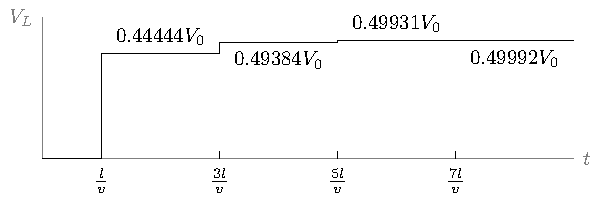
\includegraphics{figTransmissionLineTransientLoadVoltageQuestionA}
\caption{ برقی بار کی برقی دباو بالمقابل وقت۔}
\label{شکل_ترسیلی_جواب_سوال_الف}
\end{subfigure}%

\begin{subfigure}{0.8\textwidth}
\centering
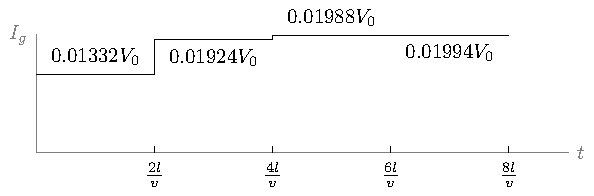
\includegraphics{figTransmissionLineTransientSourceCurrentQuestionA}
\caption{منبع کی برقی رو بالمقابل وقت۔}
\label{شکل_ترسیلی_جواب_منبع_رو_سوال_الف}
\end{subfigure}%
\caption{سوال \حوالہ{سوال_ترسیلی_بار_بردار_الف} کے خط۔}
\label{شکل_سوال_ترسیلی_سوال_الف}
\end{figure}
حل: شکل \حوالہ{شکل_سوال_ترسیلی_سوال_الف} میں دکھائے گئے ہیں۔
\انتہا{سوال}
%===========================

\ابتدا{سوال}\شناخت{سوال_ترسیلی_بار_بردار_ب}
صفحہ \حوالہصفحہ{شکل_ترسیلی_عمومی_بار_ابتدائی_موج} میں شکل \حوالہ{شکل_ترسیلی_عمومی_بار_ابتدائی_موج} دکھایا گیا ہے۔اس میں \عددی{Z_0=\SI{50}{\ohm}}،
 \عددی{R_g=R_L=\SI{100}{\ohm}} جبکہ منبع کی برقی دباو \عددی{V_0=\SI{120}{\volt}} ہے۔ لمحہ \عددی{t=0} پر سوئچ چالو کیا جاتا ہے۔\عددی{0<t<\tfrac{8l}{v}} دورانیے کے لئے بار کی برقی دباو اور  منبع کی برقی رو کے خط کھینچیں۔

\begin{figure}
\centering
\begin{subfigure}{0.8\textwidth}
\centering
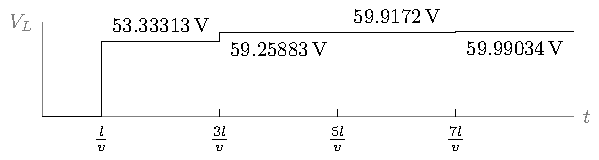
\includegraphics{figTransmissionLineTransientLoadVoltageQuestionB}
\caption{ برقی بار کی برقی دباو بالمقابل وقت۔}
\label{شکل_ترسیلی_جواب_سوال_ب}
\end{subfigure}%

\begin{subfigure}{0.8\textwidth}
\centering
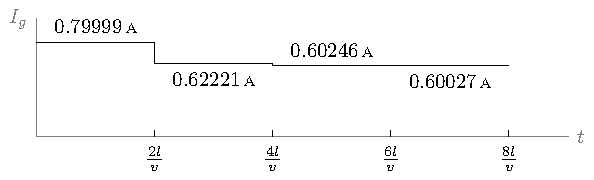
\includegraphics{figTransmissionLineTransientSourceCurrentQuestionB}
\caption{منبع کی برقی رو بالمقابل وقت۔}
\label{شکل_ترسیلی_جواب_منبع_رو_سوال_ب}
\end{subfigure}%
\caption{سوال \حوالہ{سوال_ترسیلی_بار_بردار_ب} کے خط۔}
\label{شکل_سوال_ترسیلی_سوال_ب}
\end{figure}
حل: شکل \حوالہ{شکل_سوال_ترسیلی_سوال_ب}  میں دکھائے گئے ہیں۔
\انتہا{سوال}
%===========================


\ابتدا{سوال}\شناخت{سوال_ترسیلی_بار_بردار_پ}
صفحہ \حوالہصفحہ{شکل_ترسیلی_عمومی_بار_ابتدائی_موج} میں شکل \حوالہ{شکل_ترسیلی_عمومی_بار_ابتدائی_موج} دکھایا گیا ہے۔اس میں \عددی{Z_0=\SI{50}{\ohm}}،
 \عددی{R_L=\SI{25}{\ohm}}،  \عددی{R_g=\SI{100}{\ohm}} جبکہ منبع کی برقی دباو \عددی{V_0=\SI{10}{\volt}} ہے۔تار کی لمبائی \عددی{\SI{480}{\meter}} ہے جبکہ تار میں موج کی رفتار \عددی{\SI{2.4e8}{\meter\per\second}} ہے۔ لمحہ \عددی{t=0} پر سوئچ چالو کیا جاتا ہے۔\عددی{0<t<\tfrac{8l}{v}} دورانیے کے لئے منبع سے \عددی{\SI{360}{\meter}} فاصلے پر  برقی دباو اور برقی رو کے خط کھینچیں۔

\begin{figure}
\centering
\begin{subfigure}{0.8\textwidth}
\centering
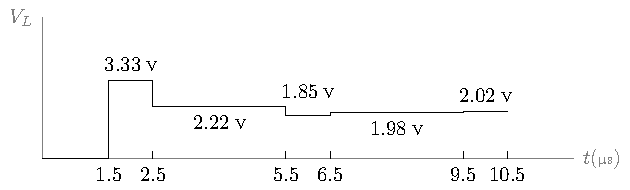
\includegraphics{figTransmissionLineTransientLoadVoltageQuestionC}
\caption{ دئے نقطے کی برقی دباو بالمقابل وقت۔}
\label{شکل_ترسیلی_جواب_سوال_پ}
\end{subfigure}%

\begin{subfigure}{0.8\textwidth}
\centering
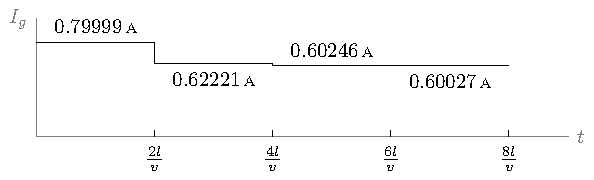
\includegraphics{figTransmissionLineTransientSourceCurrentQuestionB}
\caption{دئے نقطے کی برقی رو بالمقابل وقت۔}
\label{شکل_ترسیلی_جواب_منبع_رو_سوال_پ}
\end{subfigure}%
\caption{سوال \حوالہ{سوال_ترسیلی_بار_بردار_پ} کے خط۔}
\label{شکل_سوال_ترسیلی_سوال_پ}
\end{figure}
حل: شکل \حوالہ{شکل_سوال_ترسیلی_سوال_پ}  میں دکھائے گئے ہیں۔
\انتہا{سوال}
%===========================
